%\documentclass[]{beamer}
\documentclass[handout]{beamer}
%\usepackage[dvips]{color}
\usepackage{graphicx}
\usepackage{amsmath,amssymb,array,comment,eucal}
\newcommand{\e}{\mathbf{e}}
\renewcommand{\P}{\mathbf{P}}
\newcommand{\F}{\mathbf{F}}
\newcommand{\R}{\textsf{R}}
\newcommand{\mat}[1] {\mathbf{#1}}
%\newcommand{\ind}{\mathrel{\mathop{\sim}\limits^{\mathit{ind}}}}
%\newcommand{\iid}{\mathrel{\mathop{\sim}\limits^{\mathit{iid}}}}
\newcommand{\E}{\textsf{E}}
\newcommand{\SE}{\textsf{SE}}
\newcommand{\SSE}{\textsf{SSE}}
\newcommand{\RSS}{\textsf{RSS}}
\newcommand{\FSS}{\textsf{FSS}}
\renewcommand{\SS}{\textsf{SS}}
\newcommand{\MSE}{\textsf{MSE}}
\newcommand{\SSR}{\textsf{SSR}}
\newcommand{\Be}{\textsf{Beta}}
\newcommand{\St}{\textsf{St}}
%\newcommand{\C}{\textsf{C}}
\newcommand{\GDP}{\textsf{GDP}}
\newcommand{\NcSt}{\textsf{NcSt}}
\newcommand{\Bin}{\textsf{Bin}}
\newcommand{\NB}{\textsf{NegBin}}
\renewcommand{\NG}{\textsf{NG}}
\newcommand{\N}{\textsf{N}}
\newcommand{\Ber}{\textsf{Ber}}
\newcommand{\Poi}{\text{Poi}}
\newcommand{\Gam}{\textsf{Gamma}}
\newcommand{\BB}{\textsf{BB}}
\newcommand{\Gm}{\textsf{G}}
\newcommand{\Un}{\textsf{Unif}}
\newcommand{\Ex}{\textsf{Exp}}
\newcommand{\DE}{\textsf{DE}}
\newcommand{\tr}{\textsf{tr}}
\newcommand{\cF}{{\cal{F}}}
\newcommand{\cL}{{\cal{L}}}
\newcommand{\cI}{{\cal{I}}}
\newcommand{\cB}{{\cal{B}}}
\newcommand{\cP}{{\cal{P}}}
\newcommand{\bbR}{\mathbb{R}}
\newcommand{\bbN}{\mathbb{N}}
\newcommand{\pperp}{\mathrel{{\rlap{$\,\perp$}\perp\,\,}}}
\newcommand{\OFP}{(\Omega,\cF, \P)}
\newcommand{\eps}{\boldsymbol{\epsilon}}
\newcommand{\1}{\mathbf{1}_n}
\newcommand{\gap}{\vspace{8mm}}
\newcommand{\ind}{\mathrel{\mathop{\sim}\limits^{\rm ind}}}
\newcommand{\simiid}{\ensuremath{\mathrel{\mathop{\sim}\limits^{\rm
iid}}}}
\newcommand{\eqindis}{\ensuremath{\mathrel{\mathop{=}\limits^{\rm D}}}}
\newcommand{\iid}{\textit{i.i.d.}}
\newcommand{\SSZ}{S_{zz}}
\newcommand{\SZW}{S_{zw}}
\newcommand{\Var}{\textsf{Var}}
\newcommand{\corr}{\textsf{corr}}
\newcommand{\diag}{\textsf{diag}}
\newcommand{\var}{\textsf{var}}
\newcommand{\Cov}{\textsf{Cov}}
\newcommand{\Sam}{{\cal S}}
\def\H{\mathbf{H}}
\newcommand{\I}{\mathbf{I}}
\newcommand{\Y}{\mathbf{Y}}
\newcommand{\tY}{\tilde{\mathbf{Y}}}
\newcommand{\Yhat}{\hat{\mathbf{Y}}}
\newcommand{\Yobs}{\mathbf{Y}_{{\cal S}}}
\newcommand{\barYobs}{\bar{Y}_{{\cal S}}}
\newcommand{\barYmiss}{\bar{Y}_{{\cal S}^c}}
\def\bv{\mathbf{b}}
\def\X{\mathbf{X}}
\def\tX{\tilde{\mathbf{X}}}
\def\x{\mathbf{x}}
\def\xbar{\bar{\mathbf{x}}}
\def\Xbar{\bar{\mathbf{X}}}
\def\Xg{\mathbf{X}_{\boldsymbol{\gamma}}}
\def\Ybar{\bar{\Y}}
\def\ybar{\bar{y}}
\def\y{\mathbf{y}}
\def\Yf{\mathbf{Y_f}}
\def\W{\mathbf{W}}
\def\L{\mathbf{L}}
\def\w{\mathbf{w}}
\def\U{\mathbf{U}}
\def\V{\mathbf{V}}
\def\Q{\mathbf{Q}}
\def\Z{\mathbf{Z}}
\def\z{\mathbf{z}}
\def\v{\mathbf{v}}
\def\u{\mathbf{u}}

\def\zero{\mathbf{0}}
\def\one{\mathbf{1}}
\newcommand{\taub}{\boldsymbol{\tau}}
\newcommand{\betav}{\boldsymbol{\beta}}
\newcommand{\alphav}{\boldsymbol{\alpha}}
\newcommand{\A}{\mathbf{A}}
\def\a{\mathbf{a}}
\def\K{\mathbf{K}}
\newcommand{\B}{\mathbf{B}}
\def\b{\boldsymbol{\beta}}
\def\bhat{\hat{\boldsymbol{\beta}}}
\def\btilde{\tilde{\boldsymbol{\beta}}}
\def\tb{\tilde{\boldsymbol{\beta}}}
\def\bg{\boldsymbol{\beta_\gamma}}
\def\bgnot{\boldsymbol{\beta_{(-\gamma)}}}
\def\mub{\boldsymbol{\mu}}
\def\tmub{\tilde{\boldsymbol{\mu}}}
\def\muhat{\hat{\boldsymbol{\mu}}}
\def\t{\boldsymbol{\theta}}
\def\tk{\boldsymbol{\theta}_k}
\def\tj{\boldsymbol{\theta}_j}
\def\Mk{\boldsymbol{{\cal M}}_k}
\def\M{\boldsymbol{{\cal M}}}
\def\Mj{\boldsymbol{{\cal M}}_j}
\def\Mi{\boldsymbol{{\cal M}}_i}
\def\Mg{{\boldsymbol{{\cal M}_\gamma}}}
\def\Mnull{\boldsymbol{{\cal M}}_{N}}
\def\gMPM{\boldsymbol{\gamma}_{\text{MPM}}}
\def\gHPM{\boldsymbol{\gamma}_{\text{HPM}}}
\def\Mfull{\boldsymbol{{\cal M}}_{F}}
\def\tg{\boldsymbol{\theta}_{\boldsymbol{\gamma}}}
\def\g{\boldsymbol{\gamma}}
\def\eg{\boldsymbol{\eta}_{\boldsymbol{\gamma}}}
\def\G{\mathbf{G}}
\def\cM{\cal M}
\def\D{\Delta}
\def \shat{{\hat{\sigma}}^2}
\def\uv{\mathbf{u}}
\def\l {\lambda}
\def\d{\delta}
\def\Sigmab{\boldsymbol{\Sigma}}
\def\Lambdab{\boldsymbol{\Lambda}}
\def\lambdab{\boldsymbol{\lambda}}
\def\Mg{{\cal M}_\gamma}
\def\S{{\cal{S}}}
\def\qg{p_{\boldsymbol{\gamma}}}
\def\pg{p_{\boldsymbol{\gamma}}}
\def\t{\boldsymbol{\theta}}  
\def\T{\boldsymbol{\Theta}}  
\usepackage{verbatim}

\usetheme{Warsaw}
\usecolortheme{orchid}
\title{Estimation \& Decisions}
\institute{Merlise Clyde}
\author{STA721 Linear Models Duke University}
\date{September 24, 2014}
\logo{duke.eps}

\begin{document}
\maketitle

\begin{frame}
  \frametitle{Bayesian Estimation}
  Model
$$
\Y \sim \N(\X \b, \I_n/\phi)
$$
with precision $\phi = 1/\sigma^2$.   
\pause

\vfill
More Prior Choices:
\begin{itemize}
\item More on g-priors
\item Zellner-Siow Cauchy Prior
\item Utility and choice of Estimators
\end{itemize}
\end{frame}





\begin{frame}
\frametitle{Another Version of Zellner's $g$-prior }
\begin{eqnarray*}
\Y & = & \one \beta_0 + \X_1 \b + \eps \\
p(\beta_0, \phi) & \propto & 1 \\  
\b \mid \phi & \sim & \N(\zero, \frac{g}{\phi} (\X^T (\I_n - \P_{\one}) \X)^{-1})
\end{eqnarray*}\pause
Note $$(\X^T (\I_n - \P_{\one}) \X) = (\X^T (\I_n - \P_{\one})^T (\I_n
- \P_{\one}) \X)  = (\X -\one_n \Xbar^T)^T (\X - \one_n \Xbar) $$
\pause
Let  $(\X -\one_n \Xbar^T)^T (\X - \one \Xbar) = \SS_{\X} = \U^T \U$
\pause
Contribution quadratic to the log likelihood from prior after integrating out $\beta_0$

$$ ( \Y_c  - \X_c \b)^T(\Y_c - \X_c\b) + ( \b^T\frac{\U^T \U}{g} \b)   $$
\pause
$$ ( \Y_c  - \X_c \b)^T(\Y_c - \X_c\b) + ( \zero_p -
\frac{\U}{\sqrt{g}}\b)^T(\zero_p -  \frac{\U}{\sqrt{g}} \b)   $$

\end{frame}


\begin{frame}\frametitle{Example}

In SLR it is like an extra $Y_0 = 0$ at $\X_o = \sqrt{\frac{\SS_x}{g}}$:
$$ ( \Y_c  - \X_c \b)^T(\Y_c - \X_c\b) + (0 - \sqrt{\frac{\SS_x}{g}}\b)^T (0 - \sqrt{\frac{\SS_X}{g}} \b)   $$
\pause  
\vspace{-.25in}  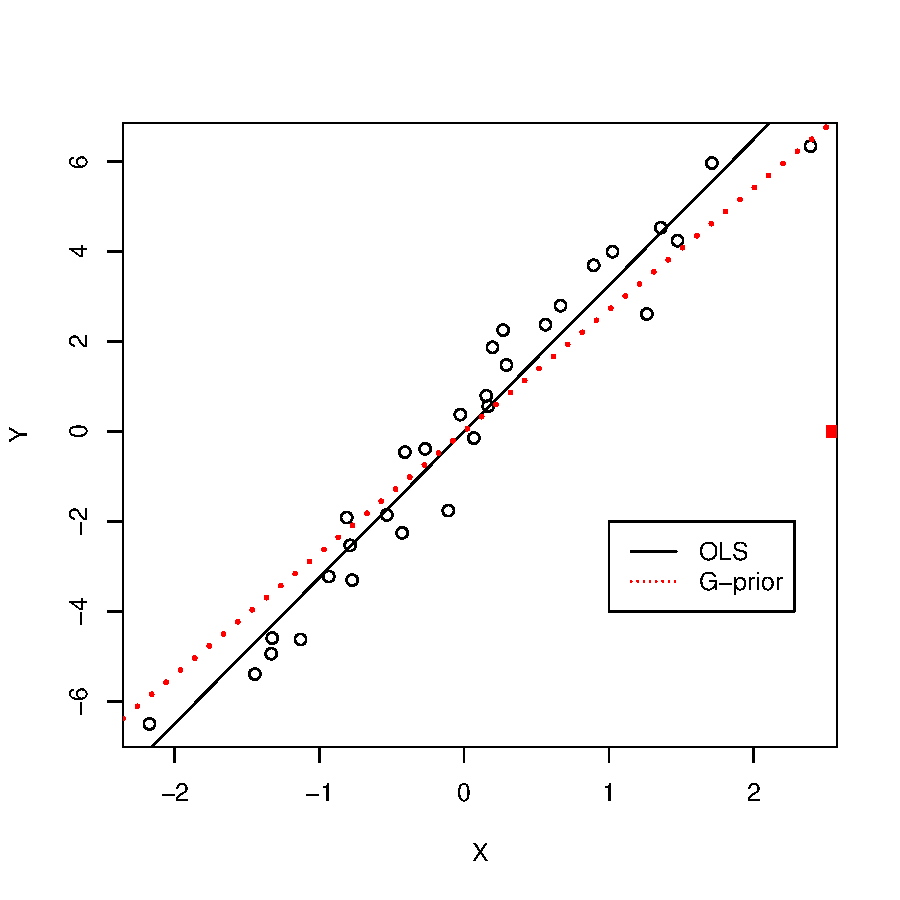
\includegraphics[height=2.75in]{gprior}
\end{frame}




\begin{frame}
  \frametitle{Disadvantages of Conjugate Priors}
  Disadvantages: \pause
\begin{itemize}
\item Results  may have be sensitive to prior ``outliers'' due to
  linear updating \pause
\item Problem potentially with all Normal priors, not just the
  $g$-prior. \pause
\item Cannot capture all possible prior beliefs \pause
\item Mixtures of Conjugate Priors
\end{itemize}
\end{frame}
\begin{frame}
  \frametitle{Mixtures of Conjugate Priors}
  \begin{theorem}[Diaconis \& Ylivisaker 1985]  Given a sampling model
  $p(y \mid \t)$ from an exponential family, any prior distribution
  can be expressed as a mixture of conjugate prior distributions 
 \end{theorem}

 \begin{itemize}
 \item Prior $p(\t) = \int p(\t \mid \omega) p(\omega)\, d \omega$ \pause
 \item Posterior \pause
   \begin{eqnarray*}
   p(\t \mid \Y)  &\propto & \int p(\Y \mid \t) p(\t \mid \omega)
   p(\omega) \, d\omega \pause \\
 & \propto & \int  \frac{  p(\Y \mid \t) p(\t \mid \omega) } {p(\Y \mid
   \omega)}  p(\Y \mid
 \omega) p(\omega ) \, d \omega  \pause \\
& \propto & \int p(\t \mid \Y, \omega)  p(\Y \mid
 \omega) p(\omega ) \, d \omega \pause \\
 p(\t \mid \Y) & =  & \frac{\int p(\t \mid \Y, \omega)  p(\Y \mid
 \omega) p(\omega ) \, d \omega }
{\int p(\Y \mid
 \omega) p(\omega ) \, d \omega }
       \end{eqnarray*}

 \end{itemize}
\end{frame}

\begin{frame}
  \frametitle{Zellner-Siow prior}
Zellner's g-prior $\b \mid \phi \sim \N(\bv_0, g n 
    (\X^T\X)^{-1}/\phi)$ \pause

\begin{itemize}
\item Choice of $g$?  \pause
\item $\frac{g}{1 + g}$  weight given to the data \pause
\item Let $\tau = 1/g$ assign $\tau \sim G(1/2, 1/2)$
\item Find prior distribution
\item Can expres posterior as a mixture of $g$-priors
\end{itemize}
\end{frame}

\begin{frame} \frametitle{Example Again}
  From JAGS:

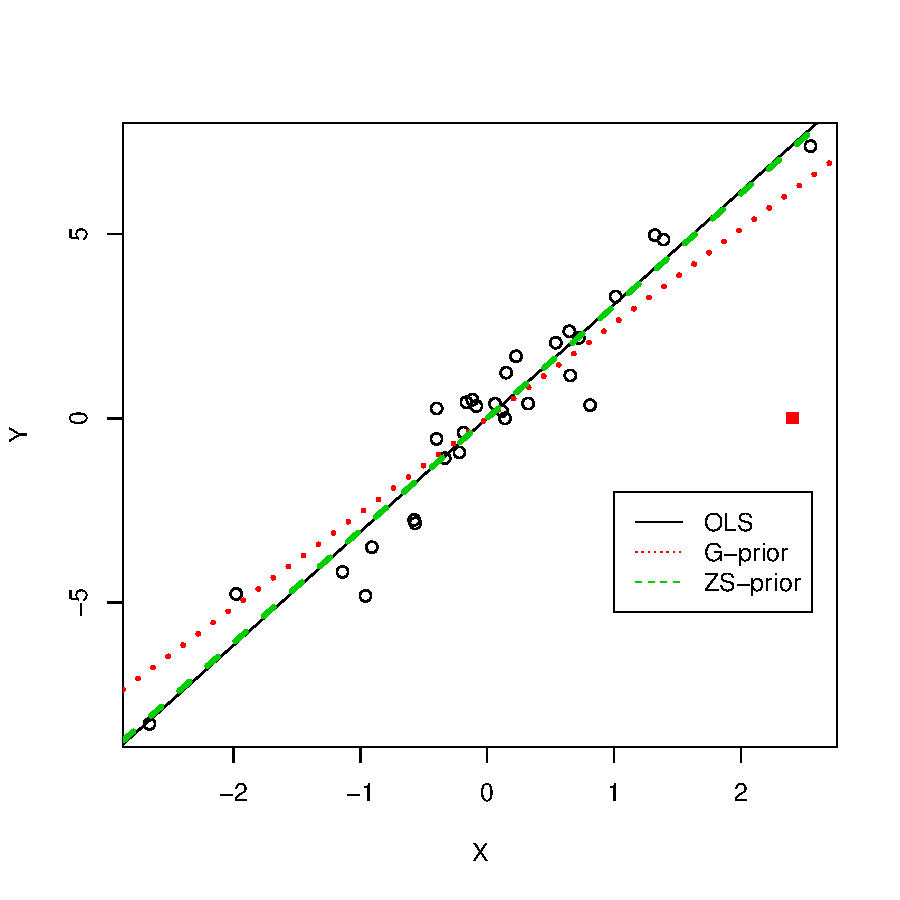
\includegraphics[height=3in]{ZSprior.pdf}

\end{frame}

\begin{frame}[fragile]{JAGS Code: library(R2jags), library(R2WinBUGS)}
\begin{verbatim}
model = function(){
  for (i in 1:n) {
      Y[i] ~ dnorm(X[i]*beta, phi)
  }
  beta ~ dnorm(0, SSX/(n*phi*lambda))
  phi ~ dgamma(.05, .05)
  lambda ~ dgamma(.5, .5)
}

write.model(model, "ZSmodel")
model.file="ZSmodel"
data = list(Y=Y, X=X, n =length(Y), SSX=sum(X^2) )
ZSout = jags(data,inits=NULL, 
             parameters.to.save=c("beta", "lambda", "phi"), 
             model=model.file, n.iter=10000)
\end{verbatim}
\end{frame}
\begin{frame}
  \frametitle{How Good are these Estimators?}
Quadratic loss for estimating  $\b$ using estimator $\a$
$$ L(\b, \a) =  ( \b - \a)^T(\b -\a)$$ \pause

\begin{itemize}
\item $a$ equals the Posterior mean $\E[\b \mid \Y]$ minimizes
  Posterior expected loss. \pause
\item Consider our expected loss (before we see the data) of taking an
``action'' $\a$ \pause
\item Under OLS or the  Reference prior the Expected Mean Square Error  \pause
  \begin{eqnarray*}
\E_\Y[( \b - \bhat)^T(\b -\bhat) & = &\sigma^2
  \tr[(\X^T\X)^{-1}] \pause \\
 & = & \sigma^2 \sum_{j=1}^p \lambda_j^{-1}
  \end{eqnarray*}
where $\lambda_j$ are eigenvalues of $\X^T\X$.
\pause
\item If smallest $\lambda_j \to 0$ then MSE  $\to \infty$
\item Note: estimate is unbiased! 
\end{itemize}
\end{frame}

\begin{frame}
  \frametitle{Is the $g$-prior better?}
  
Explore Frequentist properties of using a Bayesian estimator

$$\E_\Y[( \b - \bhat_g)^T(\b -\bhat_g)$$

but now $\bhat_g = g/(1+g) \bhat$ for $g$ prior. \pause

\vfill when is the $g$ prior better than the Reference prior of OLS?
\end{frame}

\begin{frame}\frametitle{Estimator Properties}

  \begin{itemize}
  \item  Bias  \pause
  \item  Variability \pause
  \item MSE = Bias$^2$ + Variance  (multivariate analogs) \pause
\item Problems with OLS, g-priors and mixtures of $g$-priors with collinearity \pause
\item Solutions: \pause
  \begin{itemize}
  \item removal of terms \pause
   \item other shrinkage estimators
  \end{itemize}

  \end{itemize}
\end{frame}
\end{document}

